\documentclass[german, 12pt]{book}
%\usepackage{url}
\PassOptionsToPackage{hyphens}{url}\usepackage[breaklinks=true]{hyperref}
\usepackage{dsfont}
\usepackage{listings}
\usepackage{german}
\usepackage[utf8]{inputenc}
\usepackage[final]{graphicx}
\usepackage{float}
\usepackage{geometry}
\usepackage{setspace}

\geometry{a4paper, top=30mm, left=30mm, right=20mm, bottom=35mm, headsep=10mm, footskip=12mm}


\begin{document}
	
\onehalfspacing

\title{SharkNet\\
Systembeschreibung \\
Version 0.0.6
}

\author{
Dustin Feurich
}

\maketitle

\tableofcontents

\chapter{Überblick}



\subsection{Einleitung}
Durch die rasante Entwicklung des Internet of Things (IoT) ist das Interesse an einen semantischen Datenaustausch spürbar gestiegen. Wurde in den letzten Jahrzehnten noch fast ausschließlich klassisch über die Zieladresse der Datenpakete geroutet, so werden jetzt auch die Metadaten dieser Datenpakete beim Routing zunehmend beachtet. Das Routing erfolgt hierbei inhaltsbasiert und ermöglicht ein Routing nach den Interessen der Kommunikationsteilnehmer. Der Datenaustausch zwischen diesen Teilnehmern kann beim inhaltsbasierten Routing sowohl per klassischer Client-Server Architektur, als auch über Peer-To-Peer (P2P) erfolgen. In dieser Arbeit wird der Datenaustausch über P2P erfolgen, was mehrere Vorteile bietet:
\begin{itemize}
\item Die Verbindungen zwischen Kommunikationsteilnehmern (Peers) können spontan aufgebaut werden, es wird keine Serverinfrastruktur benötigt.
\item Die Daten liegen ausschließlich bei den Peers selbst. Da es keine Zwischenstation für die Datenpakete gibt, erhöht dies die Vertraulichkeit der Kommunikation immens. 
\item Nahezu alle Kommunkationsanwendungen verwenden das Internet um den Datenaustausch zu ermöglichen. Eine Verbindung mit dem Internet ist jedoch nicht zu jeder Zeit und an jedem Ort verfügbar. Weiterhin kann auch hier auf den Zwischenservern die Kommunikation gespeichert und an Dritte weitergegeben werden.
\end{itemize}  
Der dezentrale Austausch von Daten wird unter anderem in der Android-Anwendung SharkNet realisiert. Die App verwirklicht ein dezentrales soziales Netzwerk, bei dem alle Daten ausschließlich innerhalb der Geräte gespeichert sind, es gibt keinen mithörenden zentralen Server. \\Ziel des neuen Protokolls soll es sein, dass die Benutzer der App Nachrichten an andere sich in der Nähe befindenden Benutzer versenden können. Das Routing dieser Nachrichten soll inhaltsbasiert ablaufen, so dass allein die semantische Beschreibung des Nachrichteninhalts und das Interesse der Benutzer die Route vorgibt. SharkNet hat im Kommunikationsbereich dafür einige bereits lauffähige Komponenten, für die Umsetzung des geplanten Protokolls sind aber neben der Anpassung von Alten auch neue Komponenten erforderlich. 
\newline [...]
\newpage
\subsection{Struktur}
Die Arbeit hat überwiegend einen für Informatik-Abschlussarbeiten klassischen Aufbau. Nach einer kurzen Einleitung werden die benötigten Grundlagen erläutert und anschließend wissenschaftliche Paper vorgestellt, die ein ähnliches Thema haben. Das Kapitel Entwurf erklärt den Aufbau und den Geltungsbereich des Protokolls sowie die Architektur und Oberfläche der App. Das Kapitel Implementierung beinhaltet die Komponenten, die für diese Arbeit weiterentwickelt und gänzlich neu entworfen worden sind. Die Beschreibung einer Komponente erfolgt dabei immer nach folgendem Schema:
\begin{enumerate}
	\item Es wird zunächst die Aufgabe und Bedeutung der Komponente innerhalb der App dargestellt.
	\item Anschließend wird die Architektur der Komponente mit Abbildungen vorgestellt.
	\item Darauf folgen die Hinweise, inwiefern die Komponente durch andere Softwareentwickler genutzt werden kann.
	\item Für jede Komponente gibt es außerdem ein eigenes Kapitel zum Thema Test, dies umfasst je nach Komponentenart verschiedene Testarten
	\item Abgeschlossen wird die Beschreibung der Komponente durch einen Ausblick, in dem festgehalten wird, auf welche Art und Weise die Komponente in Zukunft noch verbessert werden könnte.
\end{enumerate}
In dem sich anschließenden Kapitel Test wird ausschließlich die gesamte Anwendung getestet, die spezifischen Tests befinden sich in den Komponentenbeschreibungen. 
\newline Abgerundet wird die Arbeit durch ein abschließendes Fazit und einen Ausblick, der die Chancen und Erweiterungsmöglichkeiten der Anwendung zum Inhalt hat.
\newpage




\chapter{Verwandte Veröffentlichungen}
Es gibt zahlreiche wissenschaftliche Paper, die Semantisches oder Inhaltsbasiertes Routing zum Thema haben. Viele diese Paper sind jedoch entweder schon mindestens zehn Jahre alt, oder beinhalten nicht exklusiv den Datenaustausch über Peer-To-Peer. Im Folgenden wird jeweils die Grundidee von vier Arbeiten vorgstellt, welche ausschließlich den semantischen Datenaustausch über P2P zum Inhalt haben.\\
Strassner et. al. präsentieren ein hybrides Routing, bei dem sowohl semantisch als auch traditionell geroutet wird. Die Peers bauen hierbei ein \textit{small world} Netzwerk auf, bei dem jeder Peer viele kurze und nur wenige lange Verbindungen zu anderen Peers hat. Es werden zwei semantische Strukturen definiert - \textit{node profiles} und \textit{object profiles} - welche beide anhand von Metadaten beschrieben werden. Ein Interesse wird mit Hilfe des \textit{node profils} formuliert, das dann an die anderen Peers direkt geschickt wird. Interessiert sind die Peers an die Objekte. Durch eine semantische Ähnlichkietsanalyse wird überprüft, ob ein Peer entweder direkt ein Objekt an den anfragendne Peer liefert, oder ob er das \textit{node profile} an andere Peers weiterleitet. Das \textit{node profile} wird an den Peer weitergeleitet, bei dem die Ähnlichkeitsanalyse zwischen \textit{node profile} und \textit{object profile} am höhsten ist und sich außerdem physisch in Reichweite befindet. \\
David Faye et. al. stellen in Ihrer Ausarbeitung ein semantisches und abfrageorientiertes (Query) Routing vor. Die neuartige semantische Struktur ist hierbei die \textit{expertise table}, in der mit Metadaten festgehalten wird, welcher Peer über welches Wissen verfügt. Anders als in Sharknet sind die Peers nicht gleichberechtigt, sondern in zwei Kategorien eingeteilt: normale Peers und Super-Peers. Ein Super-Peer verwaltet mehrere normale Peers und besitzt dafür eine \textit{expertise table}. Sie reichen die Anfragen entweder an andere Super-Peers weiter oder lassen diese von normalen Peers auswerten. Ein Interesse wird mit Hilfe einer Anfrage gestellt, diese Anfrage wird durch den Routingalgorithmus an das relevante Ziel gesendet. Dies läuft folgendermaßen ab:
\begin{itemize}
	\item Ein Peer fomuliert sein Iteresse mit einer Query und sendet diese an seinen zuständigen Super-Peer, der im Paper als \textit{Godfather} bezeichnet wird.
	\item Der \textit{Godfather} wertet nun mit der Query und den \textit{expertise tables} aller verfügbaren anderen Super-Peers aus, an welche Super-Peers er die Query weiterreicht.
	\item Nachdem ein Super-Peer auf dieser Art eine Query erhalten hat, kann er diese nun entweder abermals an andere Super-Peers weiterleiten oder sie von einen seiner zugeordneten Peers ausführen lassen.
	\item Das Ergebnis der Ausführung wird nun an den eigentlichen Absender der Query zurückgeleitet.
\end{itemize}
Einen anderen Ansatz mit komplett gleichberechtigten Peers stellt Antonio Carzaniga et. al. vor, bei dem parallel zwei Protokolle ausgeführt werden. Dies umfasst zum einen das \textit{Broadcast Routing Protocol} und zum anderen das \textit{Content-based Routing Protocol}. Das Broadcast Protokoll ist für das physische Versenden der Nachrichten zwischen den Peers verantwortlich und baut eine Spanning-Tree Topologie auf. Die Nachricht wird zunächst ohne Einschränkung an alle Peers geschickt, die erreichbar sind. Das eigentliche Routing geschieht durch das \textit{Content-based Routing Protocol}. Folgende semantische Strukturen werden benutzt:
\begin{itemize}
	\item Eine \textit{Message} besteht aus typisierten Attributen
	\item Ein \textit{predicate} ist eine Disjunktion von Konjunktionen von Bedingungen (constraints), die sich auf einzelne Attribute beziehen
	\item Die \textit{content-based forwarding table} enthält die von den Peers gesetzten \textit{predicates} 	
\end{itemize}
Eine Funktion wertet anhand der \textit{forwarding table} aus, an welche Peers die Nachricht weitergeleitet werden soll. Zusätzlich wird durch das Broadcast Protokoll ermittelt, welche Peers sich physisch in Reichweite befinden. Die Nachricht wird nun alle Peers geschickt, die in beiden Mengen vorkommen. Diese Funktionsweise ähnelt SharkNet, da in der Anwendung die Nachrichten ebenfalls per Broadcast verschickt werden. Die semantische Auswertung erfolgt in SharkNet jedoch durch Profile, die vom Nutzer dynamisch festgelegt werden können und nicht durch eine sich automatisch aufbauende Tabelle. 
\\Luca Mottola et. al. haben eine sich selbst reparierende Baumtopolgie entworfen, mit der inhaltsbasiertes Routing in mobilen Ad Hoc Netzwerken realisiert werden kann. Laut Mottola et. al. benötigt eine Topologie in Form eines Baums bei ad hoc Netzwerken eine stetige Selbstreparatur, die durch das dynamische Entfernen und Hinzufügen von mobilen Geräten notwendig sei. Diese Topologie wird während der Programmausführung auf den Peers stetig angepasst, um auch bei einem häufigen Peerwechsel weiterhin benutzbar zu sein. Die Baumstruktur ist dabei für das inhaltsbasierte Routing essentiell. Das Routing erfolgt über das publish-subcribe Prinzip, wobei die Peers Nachrichten zu den Themen bekommen, die sie für die sie sich angemeldet (subscribt) haben. 
\\Der wesentliche Unterschied zwischen den vorgestellten Veröffentlichungen und dieser Arbeit sind einerseits die Eingangs- und Ausgangsprofile, mit denen natürliche Personen eingehende und ausgehende Nachrichten semantisch filtern können und andererseits die Präsentation einer konkreten mobilen Applikation, die diese Art des Routings verwirklicht. Außerdem unterscheiden sich die dafür verwendeten semantischen Strukturen deutlich von anderen Veröffentlichungen. 
\\Da diese Arbeit jedoch nicht nur das semantische Routing, sondern mit Sharknet auch ein dezentrales Netzwerk realisiert, soll an dieser Stelle kurz das bereits bekannte dezentrale soziale Netzwerk Diaspora vorgestellt werden.
\\ Jeder Benutzer kann in Diaspora einen eigenen Server benutzen, welcher als Pod bezeichnet wird. Diese Pods beinhalten die Benutzerdaten und werden vom Besitzer des Pods verwaltet. Der umfassende Datenschutz ist bei Diaspora jedoch nur dann gegeben, wenn jeder Benutzer auch einen eigenen Webserver benutzt, um damit seinen Pod zu hosten. In der Realität wird häufig aber kein eigener Webserver benutzt, außerdem ist die direkte Kommunikation zwischen den Pods nur eingeschränkt möglich. So lassen sich zum Beispiel keine Kontaktlisten von anderen Pods crawlen, auch wenn diese sie zur Verfügung stellen würden. Dies hat zur Folge, dass ein großer Teil der Benutzer sich ausschließlich mit anderen Pods verbindet, die dann zu Sammelpods werden. Diese Sammelpods entsprechen dann eher der Client-Server Architektur und nicht dezentrales P2P.
\newpage



\chapter{Grundlagen}

\subsection{Routing}
\subsubsection{Traditionelles Routing}
Routingalgorithmen werden benötigt, um Pfade für den Datenverkehr innerhalb eines Netzwerks zu finden. Beim traditionellen Routing erstellt jeder Router eine Routingtabelle, die Netzwerkadressen und Netzmasken enthält. Anhand dieser Tabelle, bei der diese Adressen auch Geräte zugeordnet sind, können dann Pakete durch das Netzwerk weitergeleitet bzw. geroutet werden. Bei der Suche nach einer geeigneten Route durch das Netzwerk wird klassischerweise ein Longest Prefix Match durchgeführt. Bei einem Treffer wird das Paket im entsprechenden output port weitergeleitet, ansonsten wird der default link genommen. Die Routingtabellen werden durch eine Analyse der vorhandenen Netzwerktopologie aufgestellt. Sollte sich die Topolgie im Betrieb ändern, muss daher auch die Routingtabelle angepasst werden. Routingschemata werden üblicherweise als Graphen dargestellt, wobei die Knoten die Kommunikationsteilnehmer und die Kanten die Leitungen zwischen den Teilnehmern darstellen. Die Kanten enthalten auch Informationen über die Kosten für die Paketübertragung zwischen Knoten. Die Kosten beziehen sich dabei meistens auf die physikalische Länge der Leitung, je länger die Leitung desto höher sind auch die Kosten. Da es bei der Wegfindung zwischen zwei nicht direkt benachbarter Knoten häufig mehrere Alternativen gibt, werden die nötigen Gesamtkosten die zwischen Anfangs- und Zielknoten auftreten, bei der Wahl des Pfades berücksichtigt. Beim traditionellen Routing wird also vorrangig nach den kostengünstigsten Pfaden zwischen Knoten innerhalb eines Netzwerks gesucht.
\\Routing-Algorithmen lassen sich in zwei Klassen aufteilen (vgl. \citet[S. 394]{Kurose2008}):
\begin{itemize}
\item Globaler Routing-Algorithmus: Hierbei ist das komplette Netzwerk bereits vor der Berechnung der kostengünstigsten Route bekannt. Es können direkt alle möglichen Pfade zwischen Ausgangs- und Zielknoten und deren Gesamtkosten bestimmt werden.
\item Dezentraler Routing-Algorithmus: Die Knoten haben hierbei nur Informationen über die Knoten und Kanten, welche sich in der Nähe befinden, das komplette Netzwerk ist nicht bekannt. Das Finden eines geeigneten Pfades kann also nur iterativ von Knoten zu Knoten geschehen und nicht bereits im Voraus.  
\end{itemize}
Da das Ziel dieser Arbeit ein semantischer Broadcast ist, bei dem sich die Kommunikationspartner vorher nicht kennen müssen, wird es sich bei dem Algorithmus um einen dezentralen Routing-Algorithmus handeln.
\\Eine weitere wichtige Unterscheidung bei Routing-Algorithmen ist die Frage, ob diese statisch oder dynamisch gestaltet sind:
\begin{itemize}
	\item Statische Routing-Algorithmen werden benutzt, wenn sich die Kanten zwischen den Knoten nur selten ändert. Die Netzwerktopologie bleibt also konstant.
	\item Bei Dynamischen Routing-Algorithmen werden bei sich häufig ändernden Netzwerktopologien eingesetzt. Sie müssen anders als die statischen Algorithmen den stetigen Wechsel von Knoten, Kanten und Kosten beachten.
\end{itemize}
Das Ergebnis dieser Arbeit wird in einer mobilen Applikation eingebunden werden und soll von natürlichen Personen per Smartphone bedient werden können. Der Routing-Algorithmus muss also zwingend dynamisch sein, da Menschen mit ihren Smartphones anders als andere Netzwerkgeräte konstant in Bewegung sind. Da bei einem Broadcast unabhängig von den Kosten die Nachricht zunächst an alle Personen geschickt werden wird, handelt es sich zusammengefasst um einen dezentralen, dynamischen und lastinsensitiven Routing-Algorithmus. 
\subsubsection{Inhaltsbasiertes Routing}
Beim inhaltsbasierten Routing wird für die Bestimmung des Pfads nicht die Zieladresse des Pakets ausgewertet, sondern die semantische Beschreibung des Paketinhalts. Jedes Paket verfügt daher über eine Inhaltsbeschreibung, wobei dann alleine von dieser Beschreibung abhängig ist, an welchen Knoten die Nachricht weitergeleitet wird (vgl. \citet[S. 649]{Tanenbaum2007}). Eine wichtige Voraussetzung für diese Art von Routing ist ein Peer-To-Peer (P2P) Netzwerk, da die Pakete stets nur von Punkt zu Punkt gesendet werden. Die Peers müssen ebenfalls ein Interesse formulieren können, anhand dessen bestimmt werden kann, ob ein Paket für sie relevant ist. Dies geschieht meist über themengesteuerte Abonnements (vgl. \citet[S. 650f]{Tanenbaum2007}). Peers können über diese Abonnements ihr Interesse an einer bestimmten Gruppe von Paketen bekunden. Es gibt zwei unterschiedliche Arten, diese Abonnements innerhalb eines Netzwerks zu verwalten:
\begin{itemize}
	\item Die Abonnements werden ausschließlich vom Peer selbst für die Auswertung herangezogen, andere Peers können diese nicht berücksichtigen. Die Pakete müssen nach der Auswertung durch den Peer dann an alle verfügbaren Peers in der Nähe weitergeleitet werden, da deren Abonnements unbekannt sind. 
	\item Die Peers teilen Ihre Abonnements den anderen Teilnehmern im Netzwerk mit. Dadurch können die Pakete nun gezielt nur an die Peers weitergeleitet werden, die sich für das Paket auch interessieren.
\end{itemize}
Beide Lösungsansätze haben Vor- und Nachteile. So hat der zweite Ansatz den Vorteil, dass nicht bei jedem Peer eine semantische Prüfung der Paketbeschreibung erfolgen muss, da diese Filterung bereits beim sendenden Peer vorgenommen worden ist. Der entscheidende Nachteil dieses Ansatzes ist jedoch, dass sämtliche Modifikationen an bestehenden Abonnements jedem Peer im Netzwerk mitgeteilt werden muss. Bei der App dieser Arbeit ist davon auszugehen, dass Benutzer ihre Abonnements (bzw. Profile) häufig editieren, was zu einer Flut an Benachrichtigungen zu anderen Peers führen könnte. Es ist bei dem Ad-Hoc Broadcast auch nicht realistisch davon auszugehen, dass jeder Peer die Abonnements der anderen Peers kennt, bevor der Benutzer eine Nachricht versendet. Da das Protokoll vorrangig von leistungsstarken Smartphones und nicht von eher leistungsschwachen Kleinstgeräten benutzt werden soll, ist der durch die wiederholte semantische Auswertung der Paketbeschreibung nötige Aufwand vernachlässigbar. In dieser Arbeit wird daher der erstgenannte Lösungsansatz verfolgt. 
\subsubsection{Broadcast-Routing}
Wenn ein Paket an alle interessierten Peers innerhalb eines Netzwerks verschickt werden soll, wird ein Broadcast-Routing benötigt, da das bisher beschriebene Unicast-Routing nur die Wegfindung zwischen zwei Knoten realisiert. Häufig sind für einen Knoten nicht alle anderen Knoten des Netzwerks direkt erreichbar, es werden also Zwischenstationen benötigt welche die Nachricht weiterleiten. Anders als beim Unicast-Routing ist die Anzahl der Pfade also variabel, je nachdem wie viele Knoten das Paket an ihre Nachbarknoten weiterleiten. Wenn ein Knoten eine Nachricht an alle Nachbarknoten schickt und diese sie wiederum an ihre Nachbarknoten schicken, wird dieser Ansatz \textit{flooding} genannt. \textit{Flooding} kann bei unbedachtem Einsatz zu Schleifen führen. Hierbei erhält und versendet ein Knoten wiederholt Nachrichten, die er bereits verwertet hat. Dieser endlose Ping-Pong-Effekt zwischen den Nachbarknoten führt dann zum sogenannten \textit{Broadcast storm}, der das gesamte Netzwerk unbrauchbar macht. \textit{Flooding} muss also zwingend kontrolliert werden, die Knoten müssen unabhängig von der semantischen Überprüfung der Nachrichten prüfen können, ob sie eine eingehende Nachricht bereits verwertet haben. In der Praxis wird meistens einer der folgenden drei Lösungsansätze für dieses Problem gewählt:
\begin{itemize}
	\item Beim sequenznummerkontrollierten \textit{Flooding} schickt jeder Knoten seine Adresse und eine Broadcast-Sequenznummer an seine Nachbarknoten. Dadurch kann jeder Knoten eine Tabelle anlegen, die bereits empfangene Pakete den Nachbarknoten zuordnet. Bei eingehenden Paketen wird nun vorher überprüft, ob dieses Paket bereits in der Liste eingetragen ist. 
	\item Das \textit{Reverse Path Forwarding} (RPF) lässt die Pakete nur dann an Nachbarknoten weiterleiten, wenn der das Paket absendende Knoten das Paket über den kürzesten Pfad erhalten hat. Es werden alle Pakete verworfen, die nicht auf dem kürzesten Unicast-Pfad zurück zur Quelle liegen. Die Nachricht wird außerdem nicht an den Nachbarknoten weitergeleitet, der auf diesen kürzesten Pfad liegt. 
	\item Der wohl bekannteste Ansatz ist der Aufbau eines \textit{Spanning Tree}, der alle Knoten genau einmal enthält. Die Knoten leiten die Nachrichten nur an ihre Baumnachbarn weiter. Dadurch können Schleifen vollständig vermieden werden.
\end{itemize}
In dieser Arbeit wird eine angepasste Variante des sequenznummerierten \textit{flooding} benutzt, um \textit{Broadcast storms} auszuschließen. Dies wird in Unterkapitel x.x genauer erläutert.

\subsection{Shark}
\subsubsection{Shark Framework}
Das Protokoll soll auf der Basis des Shark Frameworks entwickelt werden. Das Framework wurde von Prof. Dr.-Ing. Thomas Schwotzer entworfen, um die Entwicklung von semantischen Peer-To-Peer Anwendungen zu erleichtern. Es ist mit seinen semantischen Strukturen und Auswertungsmethoden für dezentrale Anwendungen geeignet. Das Wort Shark steht für Shared Knowledge - Verteiltes Wissen.
\\Das Framework definiert, dass jeder Benutzer (Peer) über eigene Wissensbasis verfügt, welche mit semantischen Annotationen versehenes Wissen des Benutzers speichert. Jede in der Wissensbasis gespeicherte Information muss daher auch semantisch beschrieben werden, bevor es in der Wissensbasis abgelegt werden kann. Informationen werden semantisch mit Wörtern beschrieben, wofür im Framework die Klasse \textit{Semantic Tag} und von dieser Klasse ableitende Klassen benutzt werden. Es werden \textit{Semantic Tags} statt normale Zeichenketten benutzt, da fast jede Sprache semantisch nicht eindeutige Wörter wie beispielsweise Homonyme aufweist. Die Tags können innerhalb von Behältern gespeichert werden, wobei es drei Arten von Behälter gibt:
\begin{itemize}
	\item \textit{Sets} enthalten \textit{Semantic Tags} ohne Beziehungen zu speichern.
	\item \textit{Taxonomies} speichern zusätzlich zu den Tags noch gerichtete Beziehungen. Diese gerichteten Beziehungen zwischen den Tags können entweder den Wert \textit{sup} oder \textit{sub} annehmen und ermöglichen somit eine hierarchische Anordnung der Wörter.
	\item Das \textit{Semantic Net} verhält sich wie eine \textit{Taxonomy}, die Beziehungen können hierbei aber beliebige Werte (in Form von Zeichenketten) annehmen. Dadurch können beispielsweise Verwandschaftsbeziehungen dargestellt werden.
\end{itemize}
Die Behälterklassen werden dann dazu benutzt, die Informationen zu beschreiben. Informationen werden mit Hilfe von sieben Dimensionen beschrieben, wobei dafür bis zu sieben Behälter und ein Literal verwendet werden.
\begin{table}[H]
	\begin{center}
		\caption{Dimensionen einer Information}
		\label{tab:dimensions}
		\begin{tabular}{l|c} 			
			Dimension & Definition \\
			\hline
			Topics & Thematische Beschreibung der Information\\
			Types & Um was für eine Art handelt es sich bei der Information\\
			Approvers & Welche Peers haben diese Nachricht \\
			Receivers & An welche Peers ist die Information gerichtet\\
			Senders & Welche Peers haben diese Nachricht versendet\\
			Locations & An welchen Orten ist diese Information relevant\\
			Times & In welchen Zeiträumen ist diese Information relevant\\
			Direction & Literal welches den Eingang und Ausgang der Information bestimmt\\
		\end{tabular}
	\end{center}
\end{table}
Dieses Unterkapitel ist nur eine rudimentäre Zusammenfassung über das Shark Framework, einen ausführlichen Überblick über das Framework bietet der Shark Developer Guide.
\subsubsection{ASIP}
Innerhalb der letzten drei Jahre wurde ein grundlegendes Protokoll für Shark entwickelt, welches die zwei zentralen Befehle bezüglich der Kommunikation zwischen Peers vorgibt und den Namen \textit{Ad hoc Semantic Internet Protocol} trägt. Die ebenfalls vom Protokoll für Shark neu eingeführten Strukturen können im entsprechenden Repository auf Github eingesehen werden.[x] In der folgenden Abbildung sind alle Bestandteile der semantischen Strukturen in ASIP abgebildet.
\begin{figure}[H]
	\centering
	\hspace*{1cm}
	\makebox[\linewidth][c]{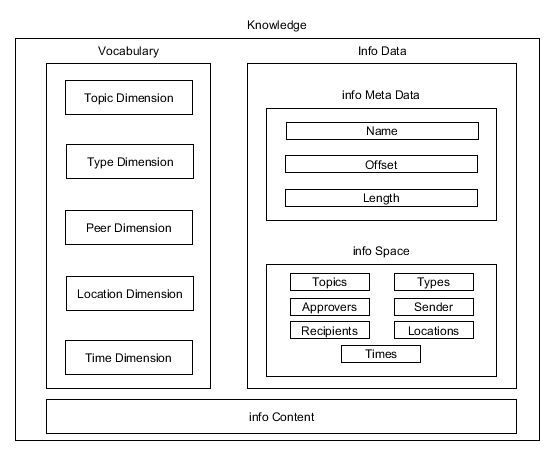
\includegraphics[width=0.9\linewidth]{general/Knowledge.png}}%
	\caption{Die ASIP/Shark Bestandtteile im Überblick}
	\label{fig:knowledge}
\end{figure}
Die beiden wichtigsten Kommandos des Protokolls sind:
\begin{itemize}
	\item Insert: Dieser Befehl wird dazu benutzt, um neue Informationen (bzw. Wissen) von anderen Peers der eigenen Wissensbasis hinzuzufügen. Dieses Wissen ist folgendermaßen unterteilt:
	\begin{itemize}
		\item Das Vokabular des Peers welches alle ihm bekannten Wörter enthält. Die Wörter sind wiederum in die fünf Dimensionen Topic, Type, Peer, Location und Time unterteilt.
		\item Der eigentliche Informationsinhalt in Form eines byte Streams mit Rohdaten.
		\item Technische Metadaten über den Informationsinhalt wie beispielsweise die Anzahl der Bytes
		\item Semantische Metadaten über den Informationsinhalt in Form der in Tabelle x.x beschriebenen sieben Dimensionen, technisch umgesetzt mit Behältern von \textit{Semantic Tags}.		
	\end{itemize} 
	\item Expose: Neben dem Hinzufügen von neuen Wissen haben Peers auch die Möglichkeit, ihr Interesse an neuem Wissen gegenüber anderen Peers zu bekunden. Dies geschieht über den Befehl \textit{Expose}, wobei auch hier das Interesse in Form der in Tabelle x.x dargestellten sieben Dimensionen formuliert wird.
\end{itemize}
[...]

\subsubsection{SharkNet}

SharkNet ist ein dezentrales soziales Netzwerk für Android Geräte und wurde von Michael Schwarz und Prof. Dr.-Ing. Thomas Schwotzer von 2015 bis 2017 entwickelt. Es kann durch die folgenden drei Kernaspekte beschrieben werden:
\begin{itemize}
	\item Dezentraler Datenaustausch ohne der Verwendung eines Servers
	\item Eine Public-Key-Infrastruktur, womit die Kommunikationspartner sich gegenseitig authentifizieren können
	\item Ausschließliche Benutzung von Open-Source Bilbiotheken und Protokollen
\end{itemize}
SharkNet bildet die Grundlage für diese Arbeit und wurde an diversen Stellen weiterentwickelt, wobei auch einige Probleme im Bereich der Kommunikation zwischen den Peers behoben werden mussten. Die ursprüngliche Zielgruppe von SharkNet sind Schüler der Katholischen Theresienschule Berlin, die als Testpersonen SharkNet anstelle von Facebook oder anderen servergebundenen sozialen Netzwerken nutzen sollten. Über die Webseite \url{http://sharedknowledge.github.io/} kann bereits ein Prototyp heruntergeladen werden, dieser enthält aber noch nicht die eigentliche Kernfunktionalität, daher keinen Chat bzw. Gruppenchat. Ein wichtiger Bestandteil dieser Arbeit ist es daher, neben dem semantischen Broadcast auch die normale Chatfunktionalität für den Endanwender benutzbar zu machen.  
\newline[...]
\newpage





\chapter{Bluetooth}


\subsubsection{Aufgabe der Komponente}
Die über SharkNet abgeschickten Nachrichten werden über Bluetooth übertragen. Die Komponente ist dabei ausschließlich für die kabellose Übertragung von Daten bzw. Nachrichten verantwortlich, die Ortung von potentiellen Kommunikationspartern erfolgt über die Wifi-Direct Komponente. Auch die Filterung von bereits bekannten oder semantisch uninteressanten Nachrichten wird nicht innerhalb dieser Komponente, sondern innerhalb der Semantischen Routing Komponente vorgenommen.
\\Da es in SharkNet neben normalen Chats auch Gruppenchats und einen semantischen Broadcast gibt, erfordert der Datenaustausch mit Bluetooth kein Pairing der miteinander kommunizierenden Geräte. Dies trägt maßgeblich zur Benutzerfreundlichkeit bei, da insbesondere beim semantischen Broadcast sonst ständig Anfragen zum Pairing auf dem Gerät erscheinen würden und vom Benutzer zusätzliche Interaktionen erforderlich wären.



\subsubsection{Architektur}

\subsubsubsection{Überlick}\label{ch:bluetoothoverview}

Im folgenden UML-Klassendiagramm sind alle Bestandteile der Bluetooth Komponente von SharkNet abgebildet.
\begin{figure}[H]
	\centering
	\hspace*{1cm}
	\makebox[\linewidth][c]{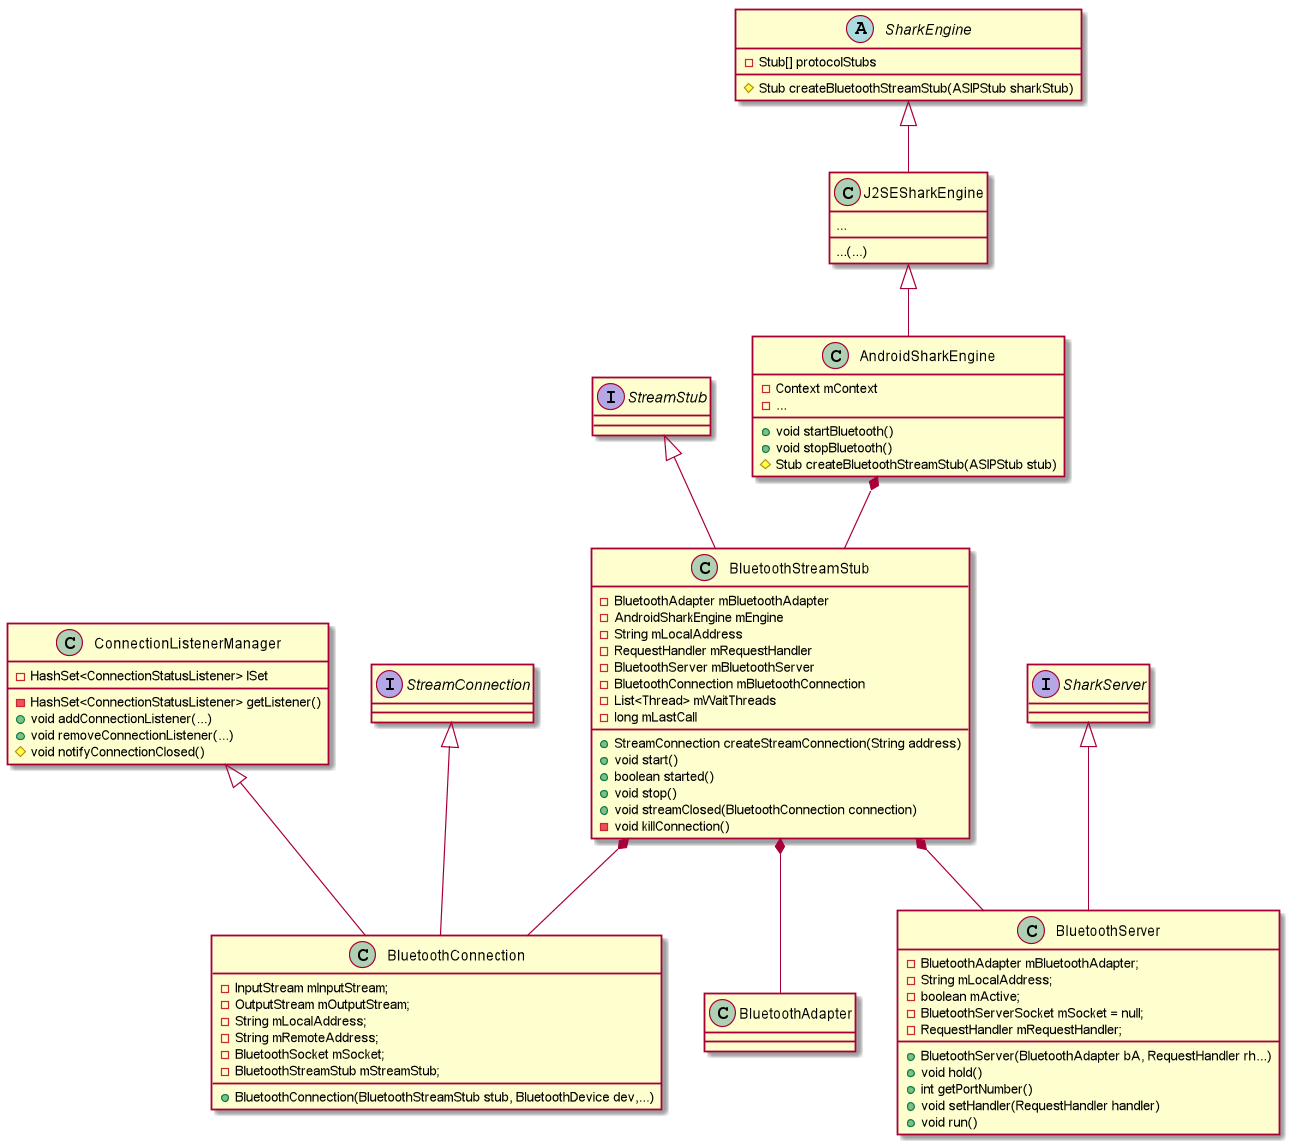
\includegraphics[width=1.1\linewidth]{bluetooth/images/bluetoothGesamt.png}}%
	\caption{Die Bluetooth Klassen im Überblick}
	\label{fig:bluetoothAll}
\end{figure}
Im Zentrum dieser Hierarchie steht die Klasse \textit{BluetoothStreamStub}. Eine Instanz dieser Klasse befindet sich als Attribut in der Klasse \textit{AndroidSharkEngine}, von der aus alle Protokolle wie NFC, Wifi-Direct oder Bluetooth gesteuert werden. Sie stellt daher auch Methoden wie \textit{startBluetooth()} oder \textit{stopBluetooth()} bereit. 





\subsubsubsection{Schnittstellendefinitionen}\label{ch:bluetoothinterfaces}
Anhand der Klassenhierarchie der Bluetooth-Komponente lässt sich erkennen, dass die folgenden drei Schnittstellen implementiert werden:
\begin{itemize}
	\item \textit{StreamStub}: Mit Hilfe von Implementierungen dieses Interfaces können streambasierte Ende-zu-Ende Verbindungen zwischen zwei Geräten hergestellt werden. Die Klasse BluetoothStreamStub öffnet und schließt daher die Verbindungen zu anderen Geräten per Bluetooth.
	\item \textit{StreamConnection}: Das Shark Framework definiert mit dem Interface StreamConnection das Verhalten einer streambasierten Verbindung zweier Geräte. Dieses Interface ist nicht zu verwechseln mit gleichnamigen Interface von Java ME. Klassen wie \textit{BluetoothConnection}, welche dieses Interface implementieren, bauen in ihren jeweiligen Konstruktur die Verbindung mit ihrem jeweiligen Protokoll auf. In der Klasse \textit{BluetoothConnection} erfolgt dies über das Bluetooth-Protokoll RFCOMM.
	\item \textit{SharkServer}: Eine dieses Interface implementierende Klassen wartet bei der bestehenden Verbindung auf Datenpakete, nimmt diese an und leitet sie an einen \textit{Request Handler} weiter. Die Klasse \textit{BluetoothServer} nimmt daher die Datenpakete an, die per bestehender Bluetoothverbindung eintreffen.

\end{itemize}

\subsubsection{Nutzung}
Der Start der Komponente erfolgt automatisch mit dem Start der Anwendung durch eine Instanzierung der Klasse \textit{AndroidSharkEngine}. Sie kann jedoch in ebenjener Klasse durch die Methoden \textit{startBluetooth()} und \textit{stopBluetooth()} auch manuell gestartet sowie gestoppt werden.

\subsubsubsection{Code}
Der Code dieser Komponente kann hier \url{https://github.com/SharedKnowledge/SharkNet-Api-Android/tree/master/api/src/main/java/net/sharksystem/api/shark/protocols/bluetooth} betrachtet werden. Wie auch die anderen Implementierungen von Über\-tra\-gungs\-pro\-to\-kol\-len, befindet sich auch die Bluetooth-Implementierung im Projekt \textit{SharkNet-Api-Android} im Package \textit{protocols}. 
\\Es werden nun die wichtigsten Codezeilen der drei im Unterkapitel Schnittstellendefinitionen erwähnten Klassen beschrieben.
\\Der \textit{BluetoothServer} horcht auf eingehende Verbindungen mit Hilfe der von Android bereitgestellten Klasse \textit{BluetoothSocket}, die folgendermaßen initialisiert wird:
 \lstset{language=Java, caption=Initialisierung des Bluetooth-Server-Sockets, label=DescriptiveLabel, numbers=left, numbersep=1em, breaklines=true, basicstyle=\small}
\begin{lstlisting}
mSocket = mBluetoothAdapter.listenUsingInsecureRfcommWithServiceRecord(BluetoothStreamStub.BT_NAME, BluetoothStreamStub.BT_UUID);
\end{lstlisting}
Hierbei wird mit Hilfe des aktiven \textit{BluetoothAdapter}, welcher auch in der Klasse \textit{BluetoothConnection} benutzt wird, über das Bluetooth-Protokoll \textit{RFCOMM} der Server-Socket erzeugt, zu dem sich andere Geräte verbinden können. Es wird statt der sonst gängigen Methode \textit{listenUsingRfcommWithServiceRecord()} die \textit{insecure} Variante genutzt, um kein Bluetooth-Pairing zwischen den Geräten vorher durchführen zu müssen. Der nächste Auszug zeigt die Annahme von eingehenden Verbindungen auf Serverseite:
 \lstset{language=Java, caption=Serverseitige Annahme der Bluetooth-Verbindungen (Auszug), label=DescriptiveLabel, numbers=left, numbersep=1em, breaklines=true, basicstyle=\small}
\begin{lstlisting}
try {
  while (mActive){
    BluetoothSocket bluetoothSocket = mSocket.accept();
    BluetoothConnection con = new BluetoothConnection(bluetoothSocket, mLocalAddress);
    mRequestHandler.handleStream(con);
  }
  mSocket.close();
\end{lstlisting}
Die Annahme der Anfrage geschieht in der dritten Zeile, wobei der daraus resultierende \textit{BluetoothSocket} in der folgenden Zeile für den Aufbau einer Verbindung genutzt wird. Die Verbindung wird anschließend vom Shark-Interface \textit{RequestHandler} verwertet. Dies bedeutet, dass die im Stream enthaltene Nachricht innerhalb der Framework-Ebene nun weiterverarbeitet wird. Dies schließt unter anderem auch die semantische Auswertung der Nachricht mit ein.
\\Der Aufbau einer Bluetooth-Verbindung erfolgt auf Clientseite ähnlich zum Aufbau auf der Serverseite innerhalb der Klasse \textit{BluetoothConnection}:
 \lstset{language=Java, caption=Clientseitige Initialisierung des Sockets, label=DescriptiveLabel, numbers=left, numbersep=1em, breaklines=true, basicstyle=\small}
\begin{lstlisting}
mSocket = device.createInsecureRfcommSocketToServiceRecord(BluetoothStreamStub.BT_UUID)
\end{lstlisting}
Auch hier wird die \textit{Insecure} Variante der Methode genommen, um auf ein Pairing verzichten zu können.
\\Instanzen der beiden bisher vorgestellten Klassen \textit{BluetoothServer} und \textit{BluetoothStreamStub} werden durch die Klasse \textit{BluetoothStreamStub} erzeugt und verwaltet. Neben der Erzeugung dieser Objekte liefert der \textit{BluetoothStreamStub} weiterhin die lokale Bluetooth MAC-Adresse des Geräts:
\textit{BluetoothConnection}:
\lstset{language=Java, caption=Auslesen der Bluetooth MAC-Adresse, label=DescriptiveLabel, numbers=left, numbersep=1em, breaklines=true, basicstyle=\small}
\begin{lstlisting}
mLocalAddress = android.provider.Settings.Secure.getString(engine.getContext().getContentResolver(), "bluetooth_address");
//mLocalAddress = BluetoothAdapter.getDefaultAdapter().getAddress() Nur vor Marshmallow nutzbar, liefert nach dieser Version nur eine unbrauchbare Konstante!
\end{lstlisting}
Dies geschieht zwangsweise über eine Reflektion, da die bis Android-Marshmallow dafür vorhergesehene Methode nur eine Konstante liefert, die nicht der eigentlichen Bluetooth MAC-Adresse des Geräts entspricht. Die Bluetooth MAC-Adresse wird jedoch zwingend für \textit{Insecure} Verbindungen benötigt, welche kein Bluetooth-Pairing erfordern, was für die Broadcast-Komponente essentiell ist. 
\\Die restlichen Methoden der Bluetooth-Komponente wie beispielsweise \textit{killConnection()} sind mnemonischer Natur.

\subsubsubsection{Deployment / Runtime}
\newline [...]


\subsubsection{Test}
\subsubsubsection{Gerätetest}
Mit den folgenden Android-Geräten ist die Komponente auf Kompatibilität geprüft worden:
\begin{table}[H]
	\begin{center}
		\caption{Kompatibilitätstest der Bluetooth-Komponente}
		\label{tab:dimensions}
		\begin{tabular}{l|c|c} 			
			Gerät & Android-Version & kompatibel \\
			\hline
			LG Nexus 5x & 8.0 & Ja\\
			LG Nexus 5x & 8.1 & Nein\\
			LG Nexus 5 & 6.1 & Ja\\
			Sony Xperia XZ Premium & 8.0 & Ja\\
			Sony Xperia Z4 Tablet & 7.1.1 & Ja\\
			Lenovo B & 6.0 & Ja\\
			Lenovo A5500-F Tablet & 4.4 & Nein\\
			Raspberry Pi 3 & 6.0.1 & Ja\\	
			Wandboard Quad & 5.0.2 & Ja\\			
		\end{tabular}
	\end{center}
\end{table}
Seit neusten Android-Version 8.1 ist es nicht mehr mit der in Listing 4.4 beschriebenen Refeklektion möglich, die Bluetooth MAC-Adresse programmatisch auszulesen. Dementsprechend kann das Testgerät Nexus 5x seit dem Update des Betriebssystems keine Nachrichten via Bluetooth mehr empfangen, da die anderen Geräte keine valide MAC-Adresse vom Nexus 5x erhalten haben und die Verbindung somit ohne Pairing nicht erfolgreich aufgebaut werden kann. 
\\Beim Lenovo A5500-F Tablet handelt es sich um eine zu alte Android-Version, wodurch in mehreren Komponenten zu Exceptions kommt, weil benötigte Methoden noch nicht enthalten sind.



\subsubsection{Ausblick}
Es ist empfehlenswert, die von Android gestellten Bluetooth Klassen durch die dazu äquivalenten Bluetooth Low Energy (BLE) Klassen entweder zu ersetzen oder zumindest eine Alternative zu dem klassischen Bluetooth Package zu bieten. BLE verbraucht weit weniger Akkuleistung als das klassische Bluetooth, kann dafür aber nur eine geringere Menge an Daten pro Verbindung unterstützen. Da die mit SharkNet verschickten Nachrichten auch trotz der semantischen Annotationen nur wenige Kilobyte benötigen, stellt dies für SharkNet kein Hindernis dar.
\\Notwendig ist zukünftig außerdem das Ersetzen der in Listing 4.4 dargestellten Reflektion zum Auslesen der Bluetooth MAC-Adresse. Dies funktioniert nur mit Geräten bis einschließlich Android 8.0, ab Android 8.1 ist die ausgelesene MAC-Adresse inkorrekt. Über die WiFi-Komponente an andere Geräte versendete inkorrekte Bluetooth-Adressen führen dann dazu, dass das Gerät keine Nachrichten über Bluetooth empfangen kann. 
\\Lasttests mit mehreren miteinander kommunizierenden Geräten und gleichzeitigem Spammen von Nachrichten haben der Komponente ebenfalls Grenzen der Belastbarkeit aufgezeigt. So können bei zu hoher Last Nachrichten verloren gehen, da das Empfangsgerät die in Listing 4.2 gezeigte \textit{accept()} Methode nicht aufgerufen wird. 
\newpage



\chapter{WiFi}
\subsubsection{Aufgabe der Komponente}
Über die WiFi-Direct Komponente vermitteln die Peers ihre Kontaktdaten an alle ver\-füg\-ba\-ren Peers in der Nähe. Dies geschieht über den Expose Befehl des ASIP Protokolls, bei dem ein ASIP-Interesse an die Wissensbasis von anderen Peers gesandt wird. Dies beinhaltet unter anderem die Bluetooth MAC-Adresse, mit der dem Peer dann anschließend Nachrichten per Bluetooth geschickt werden können. Das Übermitteln der Bluetooth Mac-Adresse via WiFi-Direct ermöglicht es daher, dass für die darauf folgende Bluetooth-Verbindung kein Pairing benötigt wird. 
\\Die Komponente ist der elementare Bestandteil des Peer-Radars, der alle sich in der Nähe befindlichen Peers anzeigt und die Kommunikation mit diesen erlaubt. Das Radar ist wiederum dafür erforderlich, neue Chats mit Peers anzulegen oder einen semantischen Broadcast ohne Bluetooth-Pairing zu ermöglichen.
\begin{figure}[H]
	\centering
	\makebox[\linewidth][c]{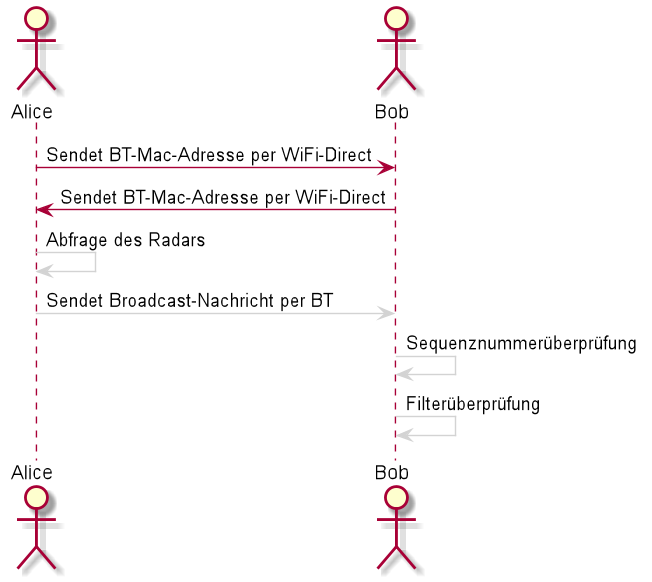
\includegraphics[width=0.6\linewidth]{wifi/images/communicationComps.png}}%
	\caption{Die WiFi Komponente innerhalb des Nachrichtenaustauschs}
	\label{fig:wifiComp}
\end{figure}
\newpage
\subsubsection{Architektur}

Im folgenden UML-Klassendiagramm sind alle Bestandteile der WiFi-Direct Komponente von SharkNet abgebildet.
\begin{figure}[H]
	\centering
	\makebox[\linewidth][c]{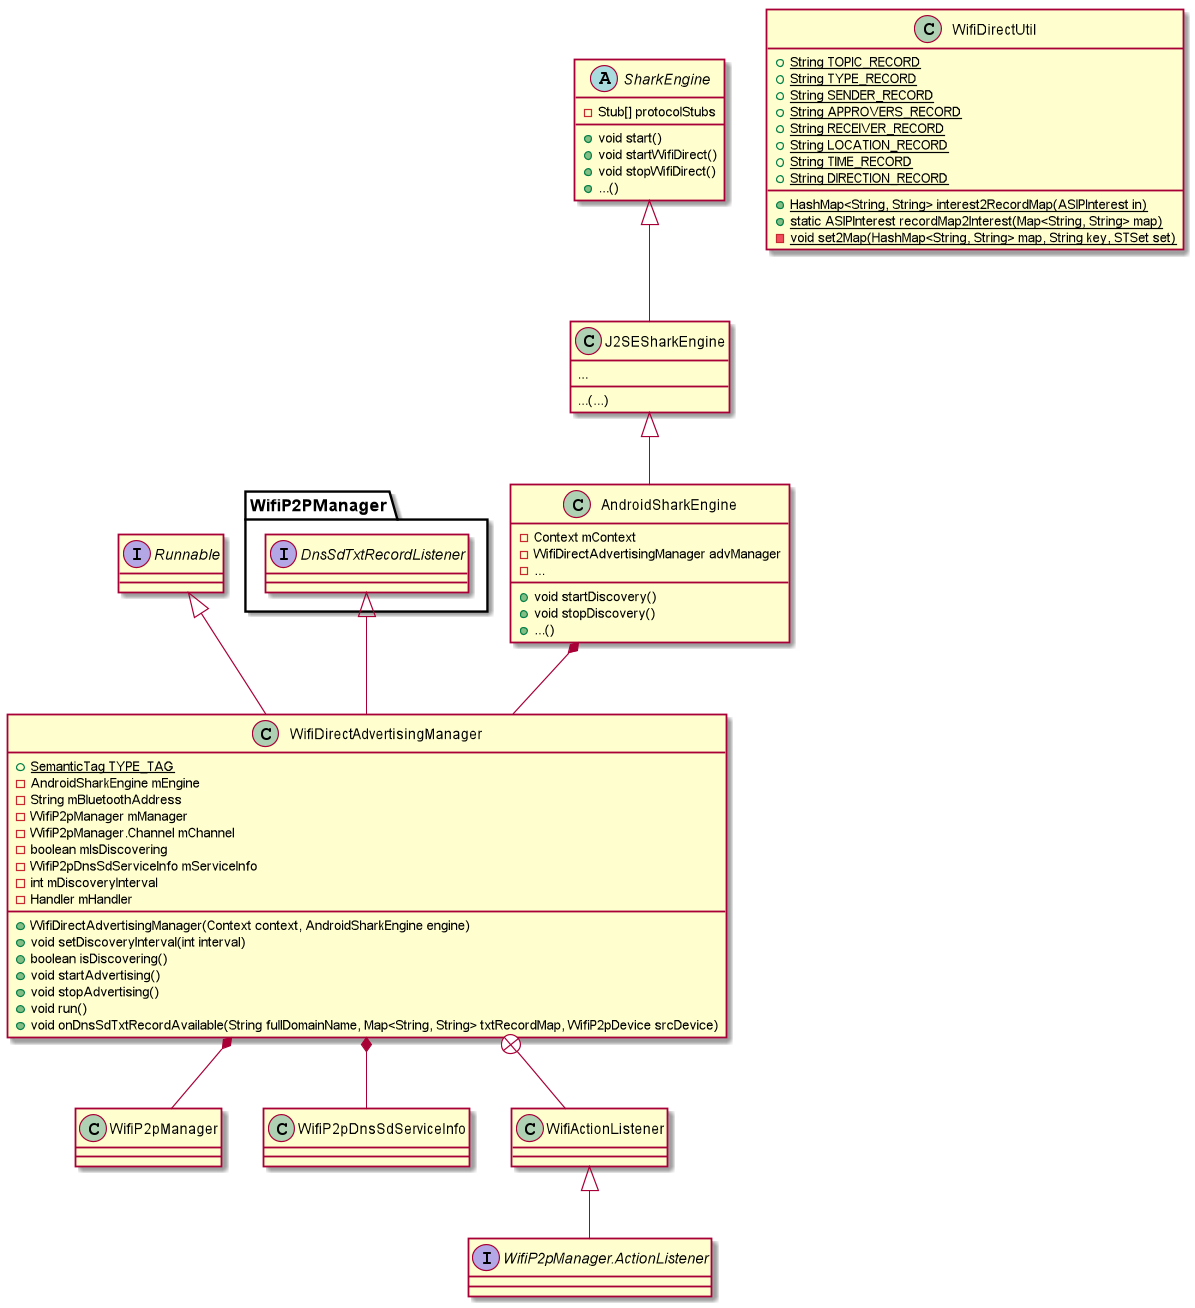
\includegraphics[width=1.1\linewidth]{wifi/images/wifiDirectGesamt.png}}%
	\caption{Die WiFi-Direct Klassen im Überblick}
	\label{fig:wifiAll}
\end{figure}
\newpage
Im Zentrum dieser Hierarchie steht die Klasse \textit{WiFiDirectAdvertisingManager}. Eine Instanz dieser Klasse befindet sich als Attribut in der Klasse \textit{AndroidSharkEngine}, von der aus alle Protokolle wie NFC, Wifi-Direct oder Bluetooth gesteuert werden. Über die Engine kann daher auch das Radar per \textit{startDiscovery()} Methode gestartet oder über die \textit{stopDiscovery()} Methode beendet werden. Das Starten oder Stoppen der kompletten WiFi-Komponente erfolgt dagegen in der Klasse \textit{AndroidSharkEngine}, die den Ausgangspunkt der Vererbungshierarchie darstellt.
\\Die Klasse \textit{WifiDirectUtil} bietet statische Methoden an, mit denen ASIP-Interessen in Hashmaps umgewandelt werden können und umgekehrt. Dies ist notwendig, da die von Android gestellte Basisklasse \textit{WifiP2PManager} bei den Anmeldungen von Services keine ASIP-Interessen, sondern Hashmaps als Parameter akzeptiert.

\subsubsection{Nutzung}
Die WiFi-Komponente wird automatisch beim Start der Anwendung gestartet. Manuell kann die Komponente über die Klasse \textit{AndroidSharkEngine} gesteuert werden, welche wie schon im Überblick erwähnt die beiden Methoden \textit{startDiscovery()} und \textit{stopDiscovery()} enthält.


\subsubsection{Code}
Der Code dieser Komponente kann unter \url{https://github.com/SharedKnowledge/SharkNet-Api-Android/tree/master/api/src/main/java/net/sharksystem/api/shark/protocols/wifidirect} betrachtet werden. Wie auch die anderen Implementierungen von Über\-tra\-gungs\-pro\-to\-kol\-len, befindet sich auch die WiFi-Direct-Implementierung im Projekt \textit{SharkNet-Api-Android} im Package \textit{protocols}.
\\Wie im vorherigen Unterkapitel erläutert, liefern die beiden Methoden \textit{startDiscovery()} und \textit{stopDiscovery()} die Funktionalität, um Peers zu finden und andere Peers über das eigene Interesse in Kenntnis zu setzen. 
\\Bei Aufruf der \textit{startDiscovery()} Methode wird innerhalb der Engine ein neuer \textit{WifiDirectAdvertisingManager} angelegt und anschließend dessen \textit{startAdvertising()} Methode aufgerufen. Innerhalb der \textit{startAdvertising()} Methode wird sich nun auf der dritten Schicht des OSI-Modells begeben, wie der folgende Codeausschnitt zeigt:\newpage
\lstset{language=Java, caption=Hinzufügung des Services, label=DescriptiveLabel, numbers=left, numbersep=1em, breaklines=true, basicstyle=\small}
\begin{lstlisting}
HashMap<String, String> map = WifiDirectUtil.interest2RecordMap(interest);
mServiceInfo = WifiP2pDnsSdServiceInfo.newInstance("_sbc", "_presence._tcp", map);
mManager.addLocalService(mChannel, mServiceInfo, new WifiActionListener("Add LocalService"));
mManager.clearServiceRequests(mChannel, new WifiActionListener("Clear ServiceRequests"));
WifiP2pDnsSdServiceRequest wifiP2pDnsSdServiceRequest = WifiP2pDnsSdServiceRequest.newInstance();
mManager.addServiceRequest(mChannel, wifiP2pDnsSdServiceRequest, new WifiActionListener("Add ServiceRequest"));
\end{lstlisting}
Nachdem in der ersten Zeile eine Hashmap aus dem Interesse erzeugt worden ist, wird diese Hashmap in Zeile zwei als Parameter für die Erzeugung einer Service Information benutzt. Anschließend wird dem \textit{WifiP2PManager} ein neuer lokaler Service hinzugefügt, wobei dieser Service die zuvor erzeugte Service Information enthält. Nachdem etwaige vorherige Service Requests beseitigt worden sind, wird der neue WifiP2P Service Request hinzugefügt. Dadurch wird nun allen Geräte in der Nähe, die auf WifiP2P Verbindungen warten, der WiFi Service Request zur Verfügung gestellt.
\\Neben dem Hinzufügen von Services, müssen diese aber auch empfangen und ausgewertet werden. Dies ist der Grund, warum der \textit{WifiDirectAdvertisingManager} das Interface \textit{Runnable} implementiert. In der dadurch implementierten Methode \textit{run()} werden die von anderen Geräten gesendeten Service Requests empfangen.\newline
\lstset{language=Java, caption=Erkennung von Services, label=DescriptiveLabel, numbers=left, numbersep=1em, breaklines=true, basicstyle=\small}
\begin{lstlisting}
mManager.discoverServices(mChannel, new WifiActionListener("Discover Services"));
mHandler.postDelayed(this, mDiscoveryInterval);
\end{lstlisting}
Sollte ein Service gefunden und erfolgreich eine Peer-To-Peer Verbindung zwischen zwei Geräten aufgebaut werden können, wird nun die aus Listing 1 bekannte Hashmap an das Gerät gesendet, welches den Service gefunden (discovered) hat. Dabei wird automatisch die Methode \textit{onDnsSdTxtRecordAvailable} aufgerufen, welche die empfangene Hashmap in ein ASIP-Interesse umwandelt und dann der Engine weiterreicht.\newline
\lstset{language=Java, caption=Vewertung des Interesses, label=DescriptiveLabel, numbers=left, numbersep=1em, breaklines=true, basicstyle=\small}
\begin{lstlisting}
ASIPInterest interest = WifiDirectUtil.recordMap2Interest(txtRecordMap);
mEngine.handleASIPInterest(interest);
\end{lstlisting}  

\subsubsection{Gerätetest}
Mit den folgenden Android-Geräten ist die Komponente auf Kompatibilität geprüft worden:\\
\begin{table}[H]
	\begin{center}
		\begin{tabular}{l|c|c} 			
			Gerät & Android-Version & kompatibel \\
			\hline
			LG Nexus 5x & 8.0 & Ja\\
			LG Nexus 5x & 8.1 & Ja\\
			LG Nexus 5 & 6.1 & Ja\\
			Sony Xperia XZ Premium & 8.0 & Ja\\
			Sony Xperia Z4 Tablet & 7.1.1 & Ja\\
			Lenovo B & 6.0 & Ja\\
			Lenovo A5500-F Tablet & 4.4 & Nein\\
			Raspberry Pi 3 & 6.0.1 & Nein\\	
			Wandboard Quad & 5.0.2 & Nein\\			
		\end{tabular}
		\caption{Kompatibilitätstest der WiFi-Komponente}
		\label{tab:dimensions}
	\end{center}
\end{table}
Die beiden Einplatinencomputer Raspberry Pi 3 und Wandboard Quad unterstützen zwar grundsätzlich WLAN, jedoch nicht WiFi-Direct. Beim Raspberry Pi 3 wäre WiFi-Direct zwar technisch möglich, benötigt aber zahlreiche Umkonfigurationen, was dadurch dann nicht mehr eine reine Android-Version darstellt. 
\\Das Lenovo A5500-F Tablet hat mit Android 4.4 eine zu alte Version, die nicht alle von der Komponente benötigten WiFi-Direct Klassen bereitstellt. 
\\Nach dem Update des LG Nexus 5x von Android 8.0 auf die Version 8.1 ist zu beachten, dass das Gerät seine Bluetooth MAC-Adresse nicht mehr programmatisch auslesen kann. Dies betrifft vor allem die Bluetooth-Komponente und wird in der dazugehörigen Komponentenbeschreibung vertieft.  

\subsubsection{Ausblick}
Die WiFi Komponente wurde SharkNet hinzugefügt, da der wiederholte Austausch von Kontakdaten zwischen den Geräten mit Bluetooth zu viel Zeit in Anspruch genommen hat. Da jedes Gerät standardmäßig alle zehn Sekunden seine Anmeldedaten an Geräte in der Nähe schickt, musste diese eher ungewöhnliche Aufteilung erfolgen. Wenn zukünftig die Bluetooth-Komponente auf Bluetooth Low Energy umgestellt werden sollte, ist es eventuell möglich, auf die WiFi Komponente zu verzichten und den gesamten Datenaustausch über Bluetooth vorzunehmen. 
\newpage

\chapter{Broadcast}
\section{Aufgabe der Komponente}
Die Broadcast Komponente ermöglicht es den Benutzern von SharkNet, Nachrichten an andere Benutzer zu schicken. Dabei können auch andere Komponenten, wie etwa der semantische Eingans- und Ausgangsfilter zum Einsatz kommen, was jedoch nicht zwingend erforderlich ist. Falls auf einen Eingangsfilter oder Ausgangsfilter verzichtet werden sollte, werden wie bei einem klassischen Broadcast die Nachrichten an alle sich in der Nähe befindlichen Geräte versendet. Inwiefern der klassische Broadcast vom Benutzer semantisch eingeschränkt werden kann, lässt sich in der Komponentenbeschreibung der Komponente Semantischer Filter in Erfahrung bringen.

\section{Architektur}

\subsection{Überlick}\label{ch:broadcastcomps}
Die folgenden Komponenten werden von der Komponente Broadcast zwingend benötigt:
\begin{itemize}
\item WifI 
\item Bluetooth 
\item Persistenz 
\end{itemize}
Optional sind hingegen die Komponenten:
\begin{itemize}
	\item Semantischer Filter
\end{itemize}

\subsection{Überlick}\label{ch:broadcastoverview}
lore

\subsection{Schnittstellendefinitionen}\label{ch:broadcastinterfaces}


\section{Nutzung}
Die Komponente ist in der App innerhalb der \textit{BroadcastActivity} eingebunden. Der Endanwender kann über die diese Activity und die dazugehörige XML-Datei die Nachrichten versenden, betrachten und mit semantischen Annotationen versehen, wobei Letzteres auch die Komponente Semantische Filter betrifft.
\\Die Komponente kann aber auch in eigenen Activities benutzt werden ohne die vorgegebene \textit{BroadcastActivity} benutzen zu müssen. Der Entwickler muss bei seiner eigenen Activity dafür lediglich von der Klasse \textit{BaseActivity} erben. Die Klasse \textit{BaseActivity} stellt das Attribut \textit{mApi} vom Typ \textit{SharkNetApi} bereit, mit dem durch die Methoden \textit{getBroadcast()} und \textit{updateBoradcast(...)} der Broadcast geliefert und verändert werden kann.

\subsection{Code}
Der Code dieser Komponente kann hier \url{https://github.com/SharedKnowledge/SharkNet/tree/master/app/src/main/java/net/sharksystem/sharknet} betrachtet werden. 

\subsection{Deployment / Runtime}



\section{Test}



\section{Ausblick}

\chapter{Semantischer Filter}
\subsubsection{Aufgabe der Komponente}
Über den Broadcast erhält der Benutzer eine Vielzahl an Nachrichten von anderen Benutzern, von denen einen Großteil für ihn irrelevant sind. Der Semantische Filter ist dafür verantwortlich, dem Benutzer nur die für ihn interessanten Nachrichten passieren und in seine Wissensbasis einfließen zu lassen. Er ist damit neben dem Broadcast die wichtigste Komponente dieser Arbeit. Neben dem bereits beschriebenen Eingangsfilter gibt es noch einen Ausgangsfilter, der für die etwaige Weiterleitung von Nachrichten an andere Peers verantwortlich ist. 
\\Die Benutzer können ihre Filter über ein Menü innerhalb des Profilbereichs einstellen, wobei dies keine Pflicht ist. Wenn keine Filter gesetzt sind, werden alle Nachrichten akzeptiert und weitergeleitet, sofern diese nicht bereits zuvor empfangen worden sind. 

\subsubsection{Architektur}

\subsubsubsection{Überlick}\label{ch:filtercomps}
Der semantische Filter gliedert sich in verschiedene Teilfilter, diese Trennung richtet sich nach den bereits bekannten Dimensionen des Shark Frameworks. Um den Gesamtfilter mit den kleineren Teilfiltern dynamisch zusammensetzen zu können, wurde das Entwurfsmuster Kompositum gewählt. Mit Hilfe dieses Musters müssen nur jeweils die Teilfilter gesetzt werden, die für den Benutzer auch eine Relevanz haben. Die folgende Klassenhierarchie verdeutlicht dieses Verhältnis:
\begin{figure}[H]
	\centering
	\hspace*{1cm}
	\makebox[\linewidth][c]{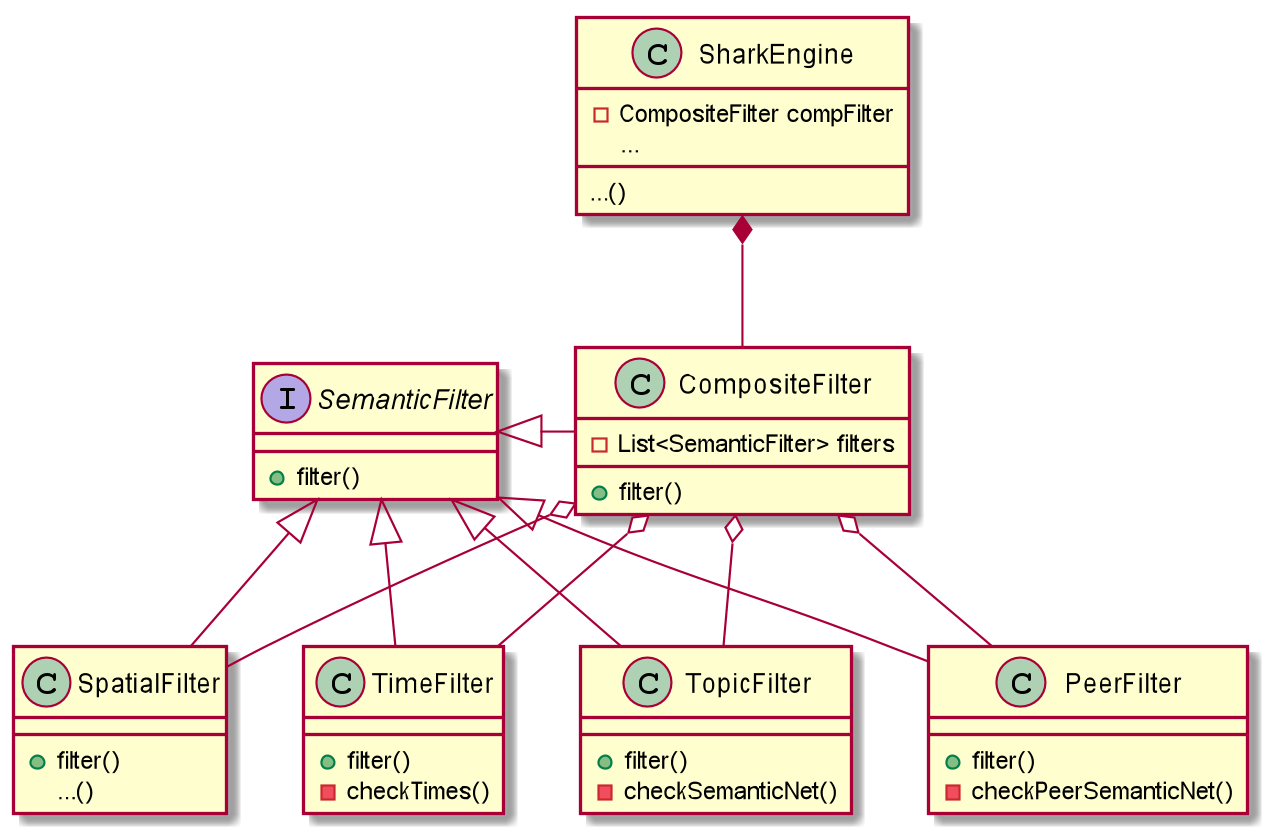
\includegraphics[width=0.6\linewidth]{semanticFilter/images/compositeFilter.png}}%
	\caption{Klassenhierarchie des semantischen Filters (Auszug)}
	\label{fig:broadcastStructure2}
\end{figure} 
\begin{itemize}
	\item Die \textit{SharkEngine} enthält das Kompositum und stellt Methoden zur Erzeugung und Anpassung dafür bereit. Weiterhin ist diese Klasse von der App aus erreichbar, wodurch über die App abhängig von den Eingaben des Benutzers die Filter gesetzt oder entfernt werden können.
	\item Das Interface \textit{SemanticFilter} wird von allen Teilfilterklassen und der Kompositumsklasse implementiert. Die einzige zu implementierende Methode ist dabei die Filtermethode, die einen booleschen Wert zurückliefert.
	\item Der \textit{CompositeFilter} besitzt, ermöglicht durch Polymorphismus, eine Liste aus allen Teilfiltern. Bei Aufruf der Filtermethode werden sämtliche Teilfilter angewandt, die sich in der Liste befinden. Näheres dazu befindet sich im Unterkapitel 7.3.1 Code. 
	\item Die Relevanz der Themen wird durch den \textit{TopicFilter} geprüft. Der Filter kann für die beiden Dimensionen Topics und Types verwendet werden.
	\item Die Dimensionen Sender, Approvers und Receivers werden durch den PeerFilter abgedeckt. Da die Dimension Sender im Gegensatz zu Approvers und Receivers nur ein SemanticTag, jedoch kein SemanticNet enthält, findet eine Fallunterscheidung am Anfang der Methode statt.
	\item Der \textit{TimeFilter} kontrolliert, ob sich mindestens einer der Zeiträume, die sich im semantischen Profil und in der empfangenen Nachricht befinden, überschneiden. 
	\item Die spatiale Auswertung findet im \textit{SpatialFilter} statt, sie wird im Rahmen einer Bachelorarbeit von Maximilian Oehme entwickelt.
\end{itemize}

\subsubsection{Code}
Wie bereits im Überblick angerissen, führt der \textit{CompositeFilter} keine eigene semantische Filterung durch, sondern lässt dies fachgerecht von den Teilfiltern ausführen. Im folgenden Codeausschnitt ist erkennbar, dass der sequentielle Aufruf der Teilfilter sofort abgebrochen wird, wenn ein Teilfilter ein \textit{false} liefert.\newline
\lstset{language=Java, caption=Filtermethode im Kompositum, label=DescriptiveLabel, numbers=left, numbersep=1em, breaklines=true, basicstyle=\small}
\begin{lstlisting}
boolean isInteresing = true;
int i = 0;
while (isInteresing && i < childFilters.size()) {
isInteresing =  childFilters.get(i).filter(message, newKnowledge, entryProfile);
i++; }
return isInteresing;
\end{lstlisting}
Angenommen es handelt sich bei der ersten Iteration der Schleife um eine Instanz der Klasse \textit{TopicFilter}, welche ihre Filtermethode aufruft, dann würde es zunächst zur folgenden Auswertung kommen:\newline
\lstset{language=Java, caption=Filtermethode des TopicType Filters (Auszug), label=DescriptiveLabel, numbers=left, numbersep=1em, breaklines=true, basicstyle=\small}
\begin{lstlisting}
if (activeEntryProfile == null) return true;
switch (dimension){
  case TOPIC:
    if (activeEntryProfile.getTopics() instanceof SemanticNet) {
	  isInteresting = checkSemanticNet(activeEntryProfile.getTopics(), newKnowledge);
	}
	else {
	  isInteresting = checkSemanticTag(newKnowledge, activeEntryProfile);
    }
break;
\end{lstlisting}
Es wird zunächst wie auch bei allen anderen Teilfiltern überprüft, ob überhaupt ein semantisches Profil vom Benutzer gesetzt worden ist. Falls nicht, wird die Auswertung sofort mit einem \textit{true} als Rückgabewert beendet. Es wird nun wie auch beim \textit{PeerFilter} überprüft, um welche Dimension es sich bei der Filterauswertung handelt. In Zeile vier von Listing 7.2 wird überprüft, ob es sich nur um ein einzelnes Tag oder um ein gesamtes SemanticNet handelt. Dadurch wird der Besonderheit in Shark Rechnung getragen, dass eine Dimension entweder durch ein einzelnes Tag oder durch ein komplettes Semantisches Netz beschrieben werden kann. Der folgende Auszug zeigt die Auswertung eines Semantischen Netzes:\newline
\lstset{language=Java, caption=Auswertung des Semantischen Netzes (Auszug), label=DescriptiveLabel, numbers=left, numbersep=1em, breaklines=true, basicstyle=\small}
\begin{lstlisting}
SemanticNet resultNet = SharkCSAlgebra.contextualize(inputNet, profileSet, fp);
	if (resultNet == null || resultNet.isEmpty()) {
		return false;
	}
	else {
		return true;
	}
\end{lstlisting}
Für die Auswertung wird die vom SharkFramework bereitgestellte Funktionalität der Kontextualisierung von Semantischen Netzen benutzt. Bei der Kontextualisierung soll das gemeinsame Interesse beider Peers bestimmt werden. Das Ergebnis der Kontextualisierung ist ein drittes Semantisches Netz, was als Fragment bezeichnet wird. Sollte dieses Fragment als Ergebnis der Prozedur nicht leer sein, haben beide Benutzer innerhalb dieser Dimension ein gemeinsames Interesse und die Nachricht wird bezüglich dieser Dimension als interessant eingestuft.
\\Die in Zeile eins dafür aufgerufene Methode benötigt dabei drei Parameter. Diese umfassen das Semantische Netz des Benutzerprofils und das Semantische Netz der Nachricht innerhalb dessen zugeordneten Dimensionen, sowie die Fragmentierungsparameter der Kontextualisierung. Die Fragmentierungsparameter werden ebenfalls vom Benutzer eingetragen und bestehen aus den folgenden drei Teilen:
\begin{itemize}
	\item Eine Liste aus erlaubten Beziehungen, welche bei der Kontextualisierung berücksichtigt werden können.
	\item Eine Liste aus nicht erlaubten Beziehungen, welche bei der Kontextualisierung nicht berücksichtigt werden.
	\item Die Tiefe, die darüber Auskunft gibt, wie viele Beziehungen zwischen den einzelnen SemanticTags berücksichtigt werden.
\end{itemize}
Nachdem das Fragment bestimmt und ausgewertet worden ist, liefert die Methode dann dementsprechend ein \textit{true} oder \textit{false} zurück. Damit ist die Auswertung der Nachricht für diese Dimension abgeschlossen.
\\Die Auswertung für die Peer Dimensionen \textit{Sender}, \textit{Receivers} und \textit{Approvers} läuft fast analog zu dem Auswertungsverfahren der Topic-Dimensionen ab. Hierbei können, falls vom Programmierer gewünscht, auch die Adressen mit ausgewertet werden. 
\\Die Auswertung der Dimension \textit{Time} ist nicht abhängig von einer Kontextualisierung, sondern von der potentiellen Überschneidung von Zeiträumen.\newline
\lstset{language=Java, caption=Auswertung der Time-Dimension (Auszug), label=DescriptiveLabel, numbers=left, numbersep=1em, breaklines=true, basicstyle=\small}
\begin{lstlisting}
while (messageTimesTags.hasMoreElements()) {
	currentMessageTag = messageTimesTags.nextElement();
		for (TimeSemanticTag currentProfileTag: profileTimesTagsList) {
			if (currentMessageTag.getFrom() > currentProfileTag.getFrom() &&
			currentMessageTag.getFrom() + currentMessageTag.getDuration() <
			currentProfileTag.getFrom() + currentProfileTag.getDuration()) {
			return true;
		}
	}
}
return false;
\end{lstlisting}
Innerhalb der Schleife werden alle \textit{TimeSemanticTags} des Profils mit denen der eingehenden Nachricht verglichen. Von der vierten bis zur sechsten Zeile werden die Zeiträume von je zwei \textit{Tags} auf Überschneidungen hin überprüft. Falls dies der Fall sein sollte, gilt die Nachricht hinsichtlich der Dimension \textit{Time} als interessant, andernfalls werden die restlichen \textit{Tags} ausgewertet. Sollte es nicht mindestens zu einer Überschneidung kommen, gilt die Nachricht gemäß der zeitlichen Dimension als uninteressant.
\\Die Auswertung der räumlichen Dimension \textit{Spatial} erfolgt durch die Aufstellung und Auswertung von Bewegungsprofilen. Diese Bewegungsprofile werden vom Smartphone (nach der Abfrage des Einverständnisses des Benutzers) aufgezeichnet und sind Teil des semantischen Profils. Nach Eingang einer Nachricht werden nun das Bewegungsprofil vom Benutzer und das Bewegungsprofil der Nachricht miteinander verglichen. Wie bereits zuvor erwähnt, ist die spatiale Auswertung der Nachrichten das Thema der Bachelorarbeit von Maximilian Oehme. Weitergehende Details und Codebeispiele können in dieser Bachelorarbeit in Erfahrung gebracht werden.

\subsubsection{Nutzung}
Die Nutzung dieser Komponente erfolgt über die zu diesem Zweck von der \textit{SharkEngine} bereitgestellten Methoden. Sie enthält wie in Abbildung 7.1 dargestellt das Kompositum, welches als Behälter dynamisch Teilfilter aufnehmen, löschen und die Reihenfolge der Ausführung ändern kann. Falls der Entwickler von der App-Ebene heraus Filter hinzufügen will, kann er dies über die \textit{SharkNetApi} tun, welche die gewünschten Änderungen an die \textit{SharkEngine} weiterleitet. Das folgende Codebeispiel zeigt diese ver\-hält\-nis\-mä\-ßig leichte Handhabung:
 \lstset{language=Java, caption=Beispiel für die Anwendung der Filter, label=DescriptiveLabel, numbers=left, numbersep=1em, breaklines=true, basicstyle=\small}
 \begin{lstlisting}
TopicFilter newTopicFilter = new TopicFilter(Dimension.TOPIC);
PeerFilter newApproverFilter = new PeerFilter(Dimension.APPROVERS);
mApi.addSemanticFilter(newTopicFilter);
mApi.addSemanticFilter(newApproverFilter);
boolean isInteresting = mApi.executeSemanticFilters(message, knowledge, profile);
 \end{lstlisting}
Nachdem die Filter erzeugt und ihre Dimension festgelegt worden sind, werden sie über die \textit{SharkNetApi} der \textit{SharkEngine} hinzugefügt und können über die Methode \textit{executeSemanticFilters()} für die Auswertung benutzt werden. Für die Auswertung muss zusätzlich die Eingangsnachricht (\textit{message}), die semantischen Annotationen der Nachricht (\textit{knowledge}) und das aktuelle semantische Profil des Benutzers (\textit{profile}) mit übergeben werden.



\subsubsection{Test}
lorem ipsum


\subsubsection{Ausblick}
lorem ipsum
\newpage

\chapter{Sonstiges}
In der folgenden Grafik sind alle Bestandteile der WifiDirect Komponente von SharkNet abgebildet.
\begin{figure}[H]
	\centering
	\hspace*{1cm}
	\makebox[\linewidth][c]{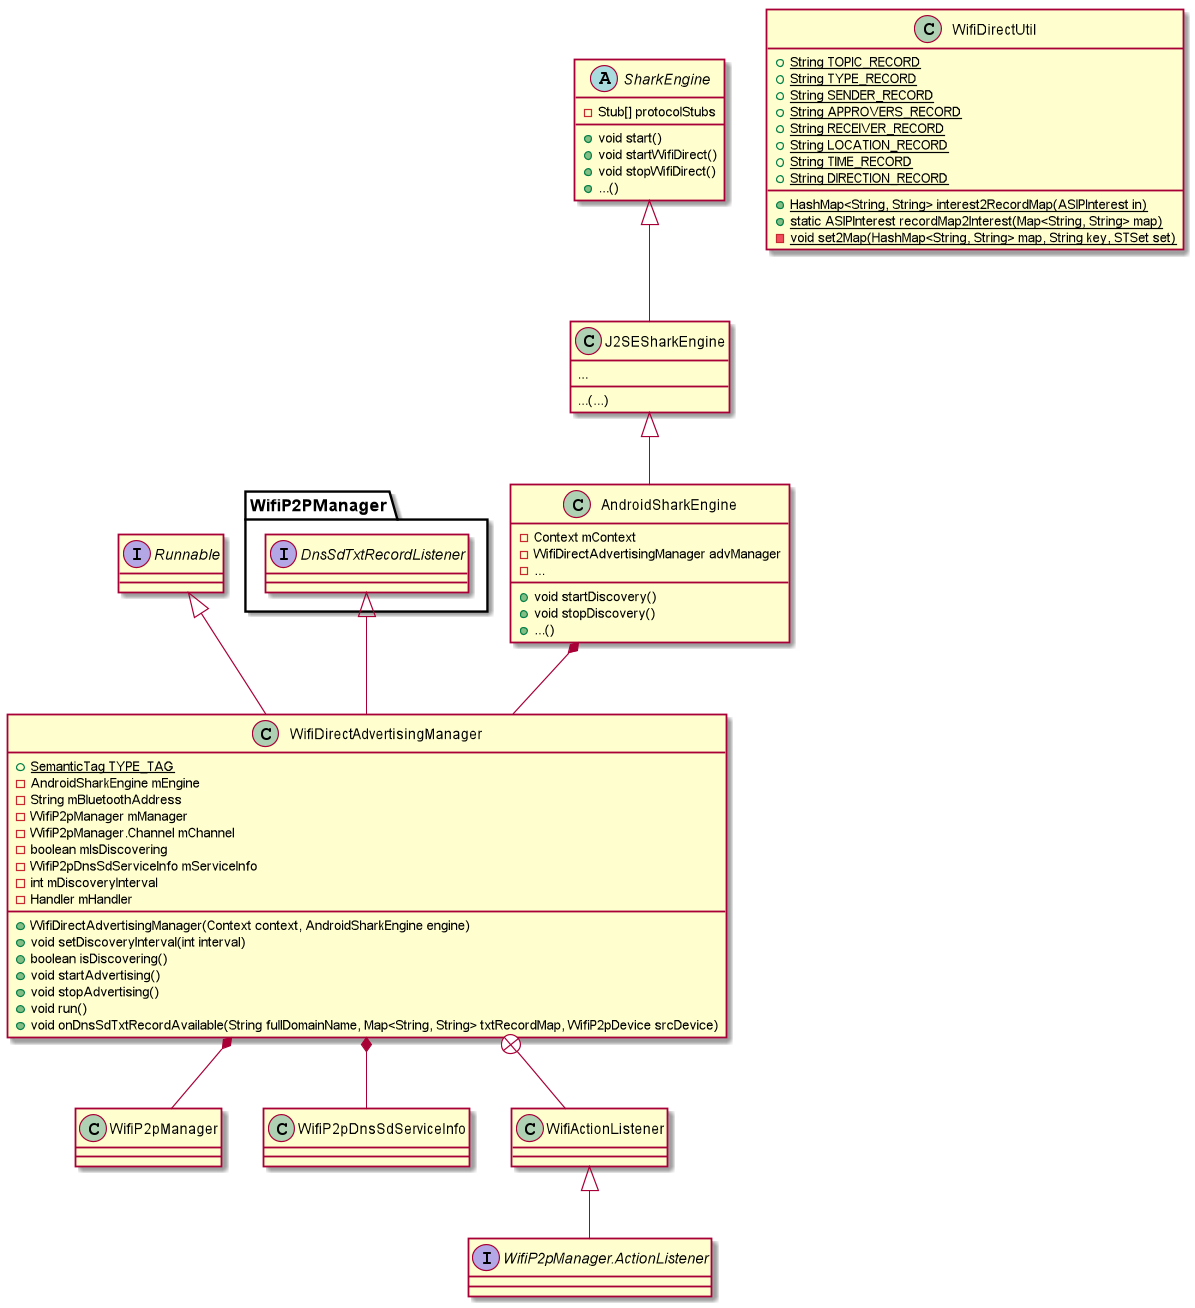
\includegraphics[width=1.1\linewidth]{wifi/images/wifiDirectGesamt.png}}%
	\caption{Die WifiDirect Klassen im Überblick}
	\label{fig:wifiAll}
\end{figure}

\newpage

In der folgenden Grafik sind alle Bestandteile der Radar Komponente abgebildet.
\begin{figure}[H]
	\centering
	\hspace*{1cm}
	\makebox[\linewidth][c]{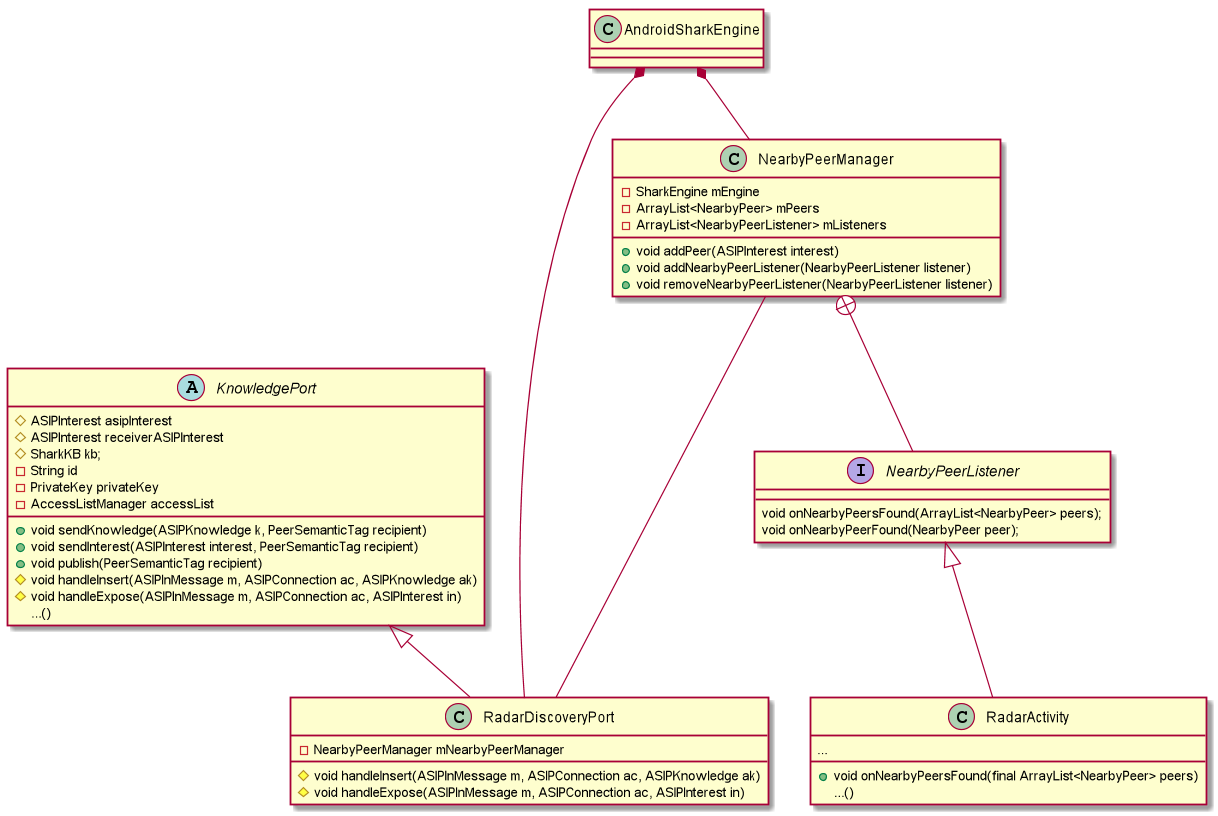
\includegraphics[width=1.1\linewidth]{bluetooth/images/radar.png}}%
	\caption{Die Radar Klassen im Überblick}
	\label{fig:radarAll}
\end{figure}

\newpage

Im folgenden Aktivitätsdiagramm wird das Versenden von Nachrichten per Broadcast abgebildet
\begin{figure}[H]
	\centering
	\hspace*{1cm}
	\makebox[\linewidth][c]{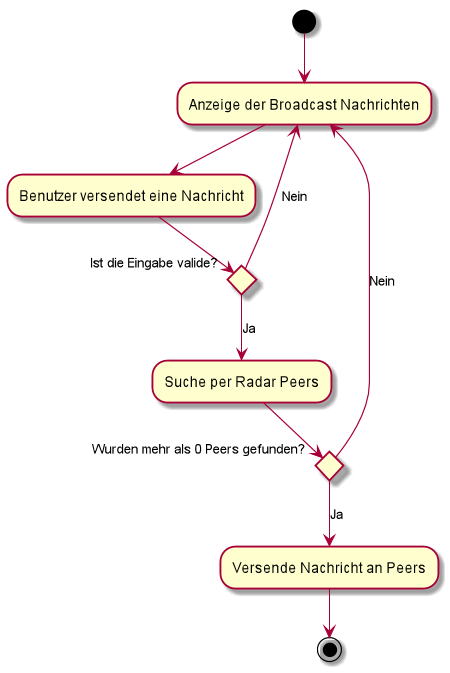
\includegraphics[width=0.5\linewidth]{broadcast/images/broadcastSend.png}}%
	\caption{Versenden von Nachrichten per Broadcast in SharkNet}
	\label{fig:broadcastSend}
\end{figure}

\newpage

Im folgenden Aktivitätsdiagramm wird das Empfangen von Nachrichten per Broadcast abgebildet
\begin{figure}[H]
	\centering
	\hspace*{1cm}
	\makebox[\linewidth][c]{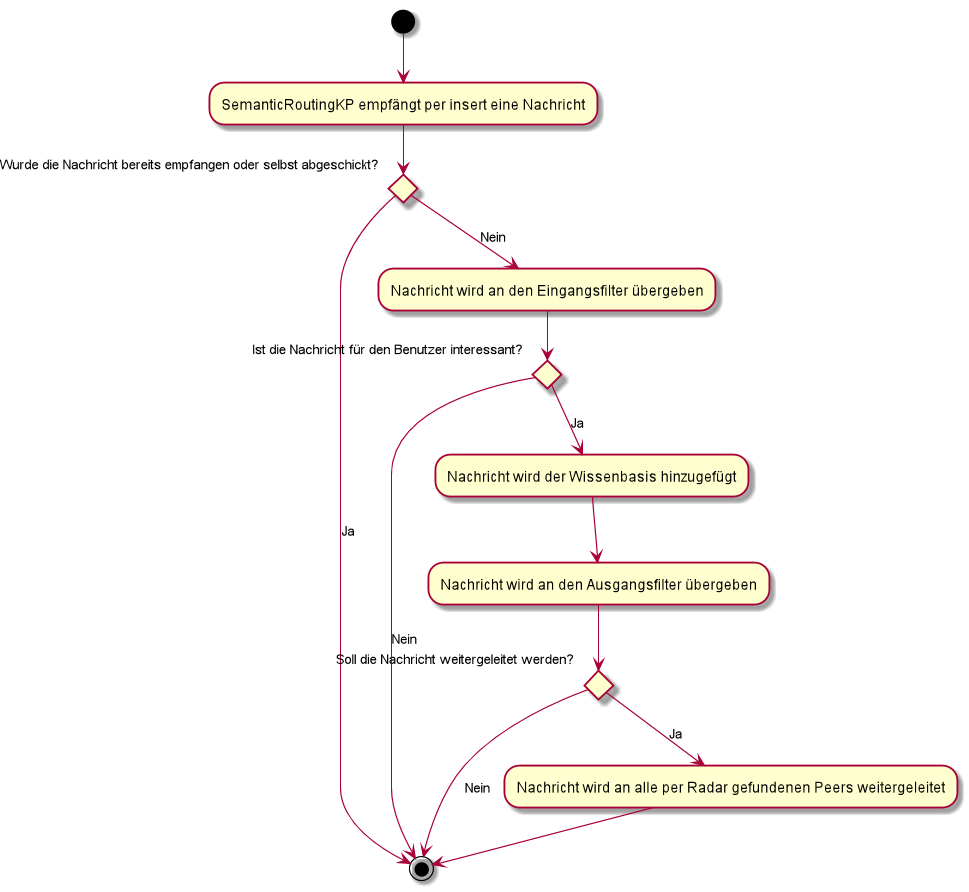
\includegraphics[width=0.9\linewidth]{broadcast/images/broadcastReceive.png}}%
	\caption{Empfangen von Nachrichten per Broadcast in SharkNet}
	\label{fig:broadcastReceive}
\end{figure}

\newpage

Im folgenden Aktivitätsdiagramm wird Filterung von Nachrichten per Eingangsfilter abgebildet
\begin{figure}[H]
	\centering
	\hspace*{1cm}
	\makebox[\linewidth][c]{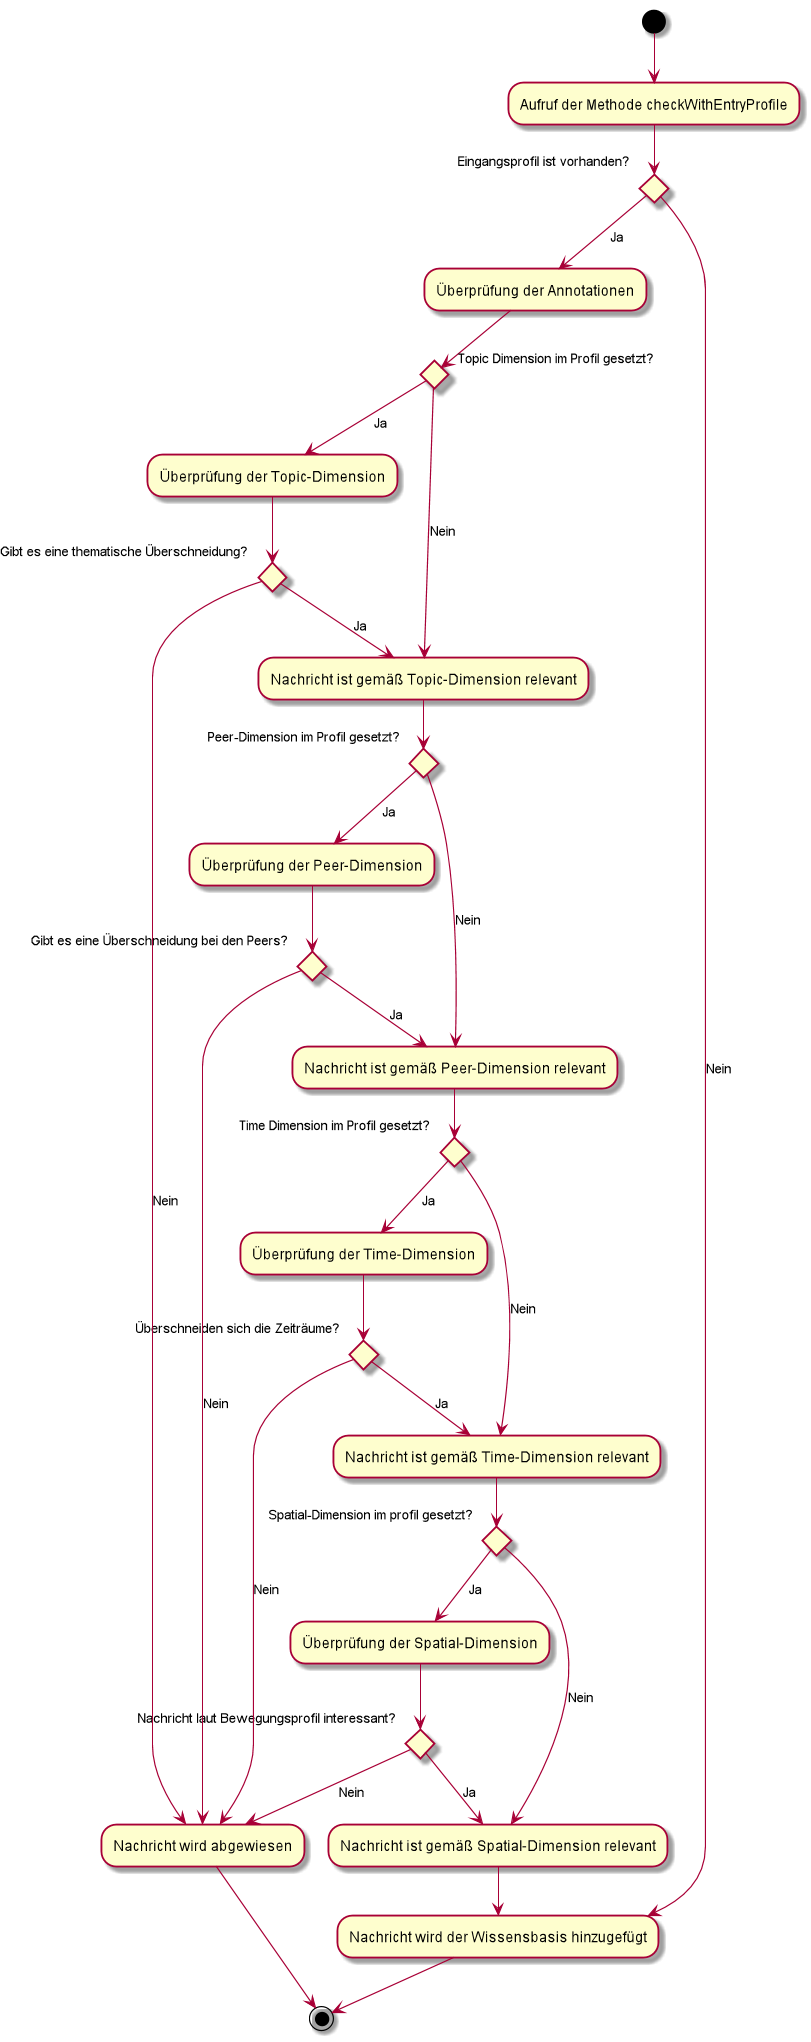
\includegraphics[width=0.6\linewidth]{broadcast/images/entryFilter.png}}%
	\caption{Filterung von Nachrichten per Eingangsfilter in SharkNet}
	\label{fig:entryFilter}
\end{figure}

\newpage

\begin{figure}[H]
	\centering
	\hspace*{1cm}
	\makebox[\linewidth][c]{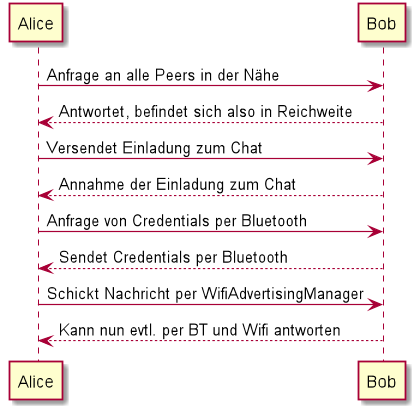
\includegraphics[width=0.7\linewidth]{broadcast/images/communication.png}}%
	\caption{Kommunikation per Chat}
	\label{fig:communication}
\end{figure}

\newpage



\end{document}